% This is samplepaper.tex, a sample chapter demonstrating the
% LLNCS macro package for Springer Computer Science proceedings;
% Version 2.20 of 2017/10/04
%
\documentclass[runningheads]{llncs}
\bibliographystyle{splncs04}
\setcounter{tocdepth}{3}
%
\usepackage{graphicx}
\usepackage{minted}
\usepackage{longtable}
% If you use the hyperref package, please uncomment the following line
% to display URLs in blue roman font according to Springer's eBook style:
% \renewcommand\UrlFont{\color{blue}\rmfamily}
\newcommand{\hs}{\mintinline{haskell}}
\usepackage{todonotes}

\begin{document}
%
\title{Concurrent oracles for free\thanks{Supported by organization x.}}
%
%\titlerunning{Abbreviated paper title}
% If the paper title is too long for the running head, you can set
% an abbreviated paper title here
%
\author{First Author\inst{1}\orcidID{0000-1111-2222-3333} \and
Second Author\inst{2,3}\orcidID{1111-2222-3333-4444} \and
Third Author\inst{3}\orcidID{2222--3333-4444-5555}}
%
\authorrunning{F. Author et al.}
% First names are abbreviated in the running head.
% If there are more than two authors, 'et al.' is used.
%
\institute{Princeton University, Princeton NJ 08544, USA \and
Springer Heidelberg, Tiergartenstr. 17, 69121 Heidelberg, Germany
\email{lncs@springer.com}\\
\url{http://www.springer.com/gp/computer-science/lncs} \and
ABC Institute, Rupert-Karls-University Heidelberg, Heidelberg, Germany\\
\email{\{abc,lncs\}@uni-heidelberg.de}}
%
\maketitle              % typeset the header of the contribution
%
\begin{abstract}
The abstract should briefly summarize the contents of the paper in
15--250 words.

\keywords{First keyword  \and Second keyword \and Another keyword.}
\end{abstract}
%
%
%
\tableofcontents
\section{Introduction and motivation}

\section{The IAM architecture and its formal model\label{sec:IAM}}
% The instruction set of IAM comprises 8 instructions. Consider the following
% instruction mnemonics and informal descriptions of their behaviour:

% \begin{longtable}{l|p{9cm}}
% \texttt{load r memaddr}     & Load a value from a memory location to a register.\\
% \texttt{loadmi r memaddr}   & Load a value from the memory location to the register using
% an indirect memory access mode\footnote{Loading the value from a memory location and using it as
% a memory address argument for the~\texttt{load} instruction.}.\\
% \texttt{set      r byte   } & Load an 8-bit immediate argument to a register.\\
% \texttt{store    r memaddr} & Store a value from a register to a memory location.\\
% \texttt{add      r memaddr} & Add a value placed in a memory location to a value contained in a register.\\
% \texttt{jump     byte     } & Perform an unconditional jump modifying the machine
% instruction counter by a given offset.\\
% \texttt{jumpz    byte     } & Performs a conditional jump if the zero flag is set.\\
% \texttt{halt              } & Stop the execution setting the halt flag.
% \end{longtable}

Figure~\ref{fig:IAMtypes} presents and encoding of the IAM microarchitecture
as a collection of Haskell types.

\begin{figure}[t]
\caption{Haskell data types encoding IAM microarchitecture.\label{fig:IAMtypes}}
\begin{minted}{haskell}
data MachineState = MachineState
    { registers           :: RegisterBank
    , instructionCounter  :: InstructionAddress
    , instructionRegister :: Instruction
    , flags               :: Flags
    , memory              :: Memory
    , program             :: Program
    , clock               :: Clock
    }

type Value = Byte

data Register = R0 | R1 | R2 | R3
type RegisterBank = Map Register Value

type MemoryAddress = Value
type Memory = Map MemoryAddress Value

data Flag = Zero
          | Halted
type Flags = Map Flag Bool

type Clock = Value
\end{minted}
\end{figure}


\section{Instruction semantics\label{sec:semantics}}
This section present a methodology of assigning IAM programs with~\emph{modular}
semantics using a~\emph{polymorphic monadic metalanguage}. We call the semantics modular because,
once encoded in the metalanguage, it may be executed in several contexts yielding
multiple different meanings of a program. In this paper we will explore (i)
state transformer semantics (section~\ref{state-trans}) to simulate program
execution and produce traces, and (ii) data dependency semantics
(section~\ref{data-deps}) allowing to derive data flow graphs from programs and
observe possible concurrent behaviour.

\subsection{Polymorphic computational metalanguage}

\begin{definition}
% \textbf{Polymorphic monadic metalanguage}
A computational metalanguage is a monad $M$ equipped with two monadic
functions: $\forall k \forall v.r: k \rightarrow M v$ and
$\forall k \forall v.w: k \rightarrow v \rightarrow M~\top$.
\end{definition}

The intuition behind this metalanguage is a concept of a~\emph{store}. A simple
store instance is a mutable variable dictionary: a data structure associating
values to keys. A value of type $v$ can be read knowing its key of type $k$,
hence the type of read function $r$ is

We embed the metalanguage in Haskell using the following type:

\begin{minted}{haskell}
data Computetion tag k v a =
     Computetion { tag         :: tag
                 , computation :: forall m. Monad m =>
                                  (k -> m v) -> (k -> v -> m ()) -> m a }
\end{minted}

A~\hs{Computation} is essentially a rank-2 polymorphic\footnote{A rank-2 polymorphic
function is one taking as a parameter another function, which is in turn (rank-1)
polymorphic. This feature requires~\hs{RankNTypes} GHC extension to be enabled.}
monadic action (denoted as~\hs{computation} here) depending on two polymorphic functions,
which we will usually name \hs{read} and~\hs{write}.
The ~\hs{tag} field contains auxiliary information which may be used for various
purposes, such as to tell apart two identical computations.

The metalanguage resembles the~\hs{MonadState} type class:

\begin{minted}{haskell}
class Monad m => MonadState s m | m -> s where
    -- | Return the state from the internals of the monad.
    get :: m s
    get = state (\s -> (s, s))

    -- | Replace the state inside the monad.
    put :: s -> m ()
    put s = state (\_ -> ((), s))
\end{minted}

A~\hs{MonadState} is a~\hs{Monad} equipped with two extra functions: the first bringing
out the current state and the second substituting it with an external one.~\hs{MonadState}
is a powerful abstraction, which allows to emulate mutable state in a pure language.
However, we would like to employ a more general, yet 

\subsection{Program simulation}

\subsection{Data dependency extraction}

\section{Deriving concurrency oracles for applicative instructions}
In this section we present a method to derive concurrency oracles from the instruction
semantics encoded in the  metalanguage (Definition~\ref{def:metalanguage}).
More specifically, we aim to reason about instructions that
have only \emph{static dependencies}.

We start by introducing formal definitions and Haskell encodings of the concepts
required for building concurrency oracles.
First, we define the notions of input and output dependencies of a computation.

\textbf{Definition (input dependency):\label{def:in-dependencies}}
Consider a term $f$ of an applicative metalanguage~\hs{Semantics Applicative a}.
A key $k$ is an~\emph{input dependency} of the term $f$ if the term $f$
performs a~\hs{read} of the key $k$.

\textbf{Definition (output dependency):\label{def:out-dependencies}}
Consider a term $f$ of an applicative metalanguage~\hs{Semantics Applicative a}.
A key $k$ is an~\emph{output dependency} of the term $f$ if the term $f$
performs a~\hs{write} of the key $k$.

\textbf{Definition (dependencies):\label{def:dependencies}}
Consider a term $f$ of an applicative metalanguage~\hs{Semantics Applicative a}.
The~\emph{dependencies} of the term $f$ are sets $I$ and $O$ -- the input and
output dependencies of the term $f$, respectively.

In the Haskell implementation, we do not distinguish between input and output dependencies
in the type level, thus the function determining the dependencies of a computation
has the following type:

\begin{minted}[xleftmargin=10pt]{haskell}
dependencies :: Semantics Applicative a -> Maybe ([Key], [Key])
\end{minted}

\noindent
The~\hs{Maybe} type constructor comes from the definition of the metalanguage:
if the applicative semantics is partial (returns~\hs{Nothing}) it is impossible
to extract its static dependencies. Successful static analysis yields a pair of
lists representing the sets of input and output dependencies of a computation.

To extract the static data dependencies of an applicative computation we need to
interpret its semantics in the special context of a \emph{constant functor}.

\subsection{The constant functor}

The~\hs{Const a b} data type is defined as follows~\cite{Mcbride:2008:APE:1348940.1348941}:

\begin{minted}[xleftmargin=10pt]{haskell}
newtype Const a b = Const { getConst :: a }
\end{minted}

\noindent
A value of the~\hs{Const a b} is just a value of any type~\hs{a}
wrapped in a data constructor. However, it is important that the type constructor
has a~\emph{phantom type} variable. This type variable allows us to
declare useful instances of standard Haskell type classes such as~\hs{Functor}
and \hs{Applicative} for \hs{Const a}. We would like to use this data type as a
computational context for applicative semantics, hence we declare the
corresponding instance\footnote{\hs{Const a} also has a \hs{Functor} instance,
where~\hs{fmap _ (Const x) = Const x}.}:

\begin{minted}[xleftmargin=10pt]{haskell}
instance Monoid m => Applicative (Const m) where
    pure _              = Const mempty
    Const x <*> Const y = Const (x `mappend` y)
\end{minted}

This instance exactly describes the desired behaviour of static dependency tracking
computational context.~\hs{Const [Key]} is an applicative functor that ignores
its enclosed value, but accumulates the declared dependencies using the~\hs{Monoid}
instance for Haskell list data type\footnote{The empty list~\hs{[]} is the
monoid identity element and the list concatenation~\hs{(++)} is the associative
binary operation.}.

\subsection{Extracting dependencies}

Using the seemingly vacuous datatype \hs{Const} we define the
function \hs{dependencies}:

\begin{minted}[xleftmargin=10pt]{haskell}
dependencies :: Semantics Applicative a -> Maybe ([Key], [Key])
dependencies s = partitionEithers . getConst <$> s read write
  where read  k    =       Const [Left  k]
        write k fv = fv *> Const [Right k]
\end{minted}

\noindent
We instantiate the polymorphic computation context with \hs{f = Const [Key]}
and supply custom tracking \hs{read} and \hs{write} functions. In fact, \hs{read}
does not perform any reading and just tracks the key as an input dependency,
whereas \hs{write} tracks the key as an output dependency and executes the
effectful computation \hs{fv}, to appropriately track its dependencies. The
resulting list of keys gets unwrapped and unzipped by standard
\hs{partitionEithers}~\hs{.}~\hs{getConst}.

This whole paper is built around the above three-line implementation of the
function \hs{dependencies}: the rest is just functional programming background
and folklore, which is required for understanding these three lines of code.

Fully armed with static dependency analysis, we can now define concurrency
oracles for programs written in the presented metalanguage.

\subsection{Concurrency oracle}
% \vspace{-2em}
A concurrency oracle is a function taking two computations and statically
determining if they are data~\emph{concurrent}, i.e. do not share any
data dependencies.


\textbf{Definition (Concurrency Oracle Answer):\label{def:concurrency-status}}
Two terms of the metalanguage are \emph{concurrent} if they do not share any
data dependencies. They are in a \emph{read} or \emph{write conflict} if they
share any input or output dependencies, respectively. If the share both input
and output dependencies then they are considered to be in a \emph{read-write
conflict}. We use the following data type is used to encode concurrency oracle
answers:

\begin{minted}[xleftmargin=10pt]{haskell}
data OracleAnswer k = Concurrent
                    | ReadConflict [k]
                    | WriteConflict [k]
                    | ReadWriteConflict [k]
\end{minted}

\textbf{Definition (concurrency oracle):\label{def:oracle}}
Consider two terms with applicative semantics \hs{s1} and \hs{s2} of the
type~\hs{Semantics Applicative a}. A~\emph{concurrency oracle} is a
function of the following type:
% \vspace{-3em}
\begin{minted}[xleftmargin=10pt]{haskell}
concurrencyOracle :: Eq k => Semantics Applicative k v1 a
                          -> Semantics Applicative k v2 a
                          -> Maybe (OracleAnswer k)
\end{minted}

\noindent
The function is required to return \hs{Nothing} when one of the given semantics
is undefined, e.g. if it corresponds to an instruction with dynamic dependencies.
Below is one possible implementation:

\begin{minted}[xleftmargin=10pt]{haskell}
concurrencyOracle s1 s2 = do
    (r1, w1) <- dependencies s1
    (r2, w2) <- dependencies s2
    let readConflicts      = intersect r1 r2
        writeConflicts     = intersect w1 w2
        readWriteConflicts = intersect (r1 ++ w1) (r2 ++ w2)
    pure $ case (readConflicts, writeConflicts, readWriteConflicts) of
        ([], [], [] ) -> Concurrent
        (rs, [], rws) | rs == rws -> ReadConflict rs
        ([], ws, rws) | ws == rws -> WriteConflict ws
        (_ , _ , rws) -> ReadWriteConflict rws
\end{minted}
% \vspace{-3em}

The oracle determines static dependencies of two given terms and examines
several possible cases of the intersections of their input and output
dependencies.

\subsection{Example oracles}

In this subsection we show two examples to illustrate the usage of concurrency
oracles. The examples are given in the form of interactive sessions, where
`\hs{ghci>}' denotes the command prompt.

Two \hs{Load} instructions with different arguments are concurrent as confirmed
by the oracle returning the result \hs{Just Concurrent}:

\begin{minted}[xleftmargin=10pt]{haskell}
ghci> concurrencyOracle (semanticsA (Load R0 0))
                        (semanticsA (Load R1 1))
Just Concurrent
\end{minted}

\noindent
Extending the first computation with an additional \hs{Add} instruction causes
a read conflict, as desired:
\begin{minted}[xleftmargin=10pt]{haskell}
ghci> p1 = blockSemanticsA [Load R0 0, Add R0 1]
ghci> p2 = semanticsA (Load R1 1)
ghci> concurrencyOracle p1 p2
Just (ReadConflict [Addr 1])
\end{minted}

\noindent
We can overlay dependency graphs of programs \hs{p1} and \hs{p2} as follows (we
place the programs at starting addresses 10 and 20, respectively):

\begin{minted}[xleftmargin=10pt]{haskell}
ghci> Just g1 = programDataGraph (zip [10..] [Load R0 0, Add R0 1])
ghci> Just g2 = programDataGraph (zip [20..] [Load R1 1])
ghci> drawGraph (overlay g1 g2)
\end{minted}

\noindent
The resulting dependency graph is shown in Fig.~\ref{fig-example-graph}.
% In the graph, instructions labelled with 1 and 2 belong to the blocks~\hs{p1}
% and~\hs{p2} respectively.
As one can see, the programs have a read conflict on key \hs{Addr 1},
just like the oracle has determined.

\begin{figure}
\vspace{-4mm}
\centerline{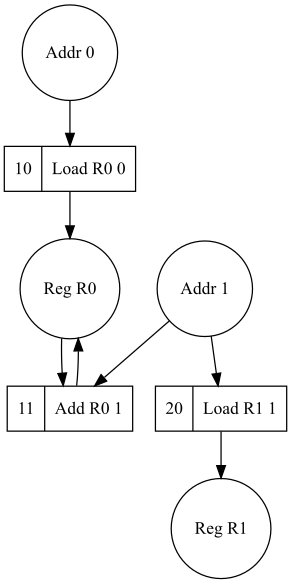
\includegraphics[scale=0.6]{img/oracle2.pdf}}
\vspace{-3mm}
\caption{An overlay of static dependency graphs of two blocks of instructions.\label{fig-example-graph}}
\vspace{-9mm}
\end{figure}


\section{Case study}

\section{Conclusion}
%
% ---- Bibliography ----
%
% BibTeX users should specify bibliography style 'splncs04'.
% References will then be sorted and formatted in the correct style.
%
\bibliography{biblio}
\end{document}
